\chapter{Methodology}\label{chapter:Methodology}

The following part explains the single steps of the forecasting process for this Interdisciplinary Project in detail.The forecast will be presented from the very beginning.\newline
First of all, the problem will be defined properly. Then the information needed will be specified and gathered. This data is then analyzed in a preliminary step and after this models for the data will be examined. In the end the result of the models will be evaluated and further proceeding will be explained in the final conclusion.
\section{Section One}\label{section:Section One}
\subsection{Subsection One}\label{labelname}

Refer to symbols or abbreviations with\\\verb+\gls{symbolname} \glstext{symbolname} \glsfirst{symbolname}+:\\
\gls{symb:N} \glstext{symb:N} \glsfirst{symb:N}\\
\gls{BA} \gls{DA} \gls{MA}

Refer to other sections with \verb+\ref{labelname}+:\\
A reference to this subsection: \ref{labelname}

Include figures with\\
\verb+\begin{figure}+\\
\verb+...+\\
\verb+\caption{An example figure}\label{fig:example}\end{figure}+

\begin{figure}[h]
\begin{center}
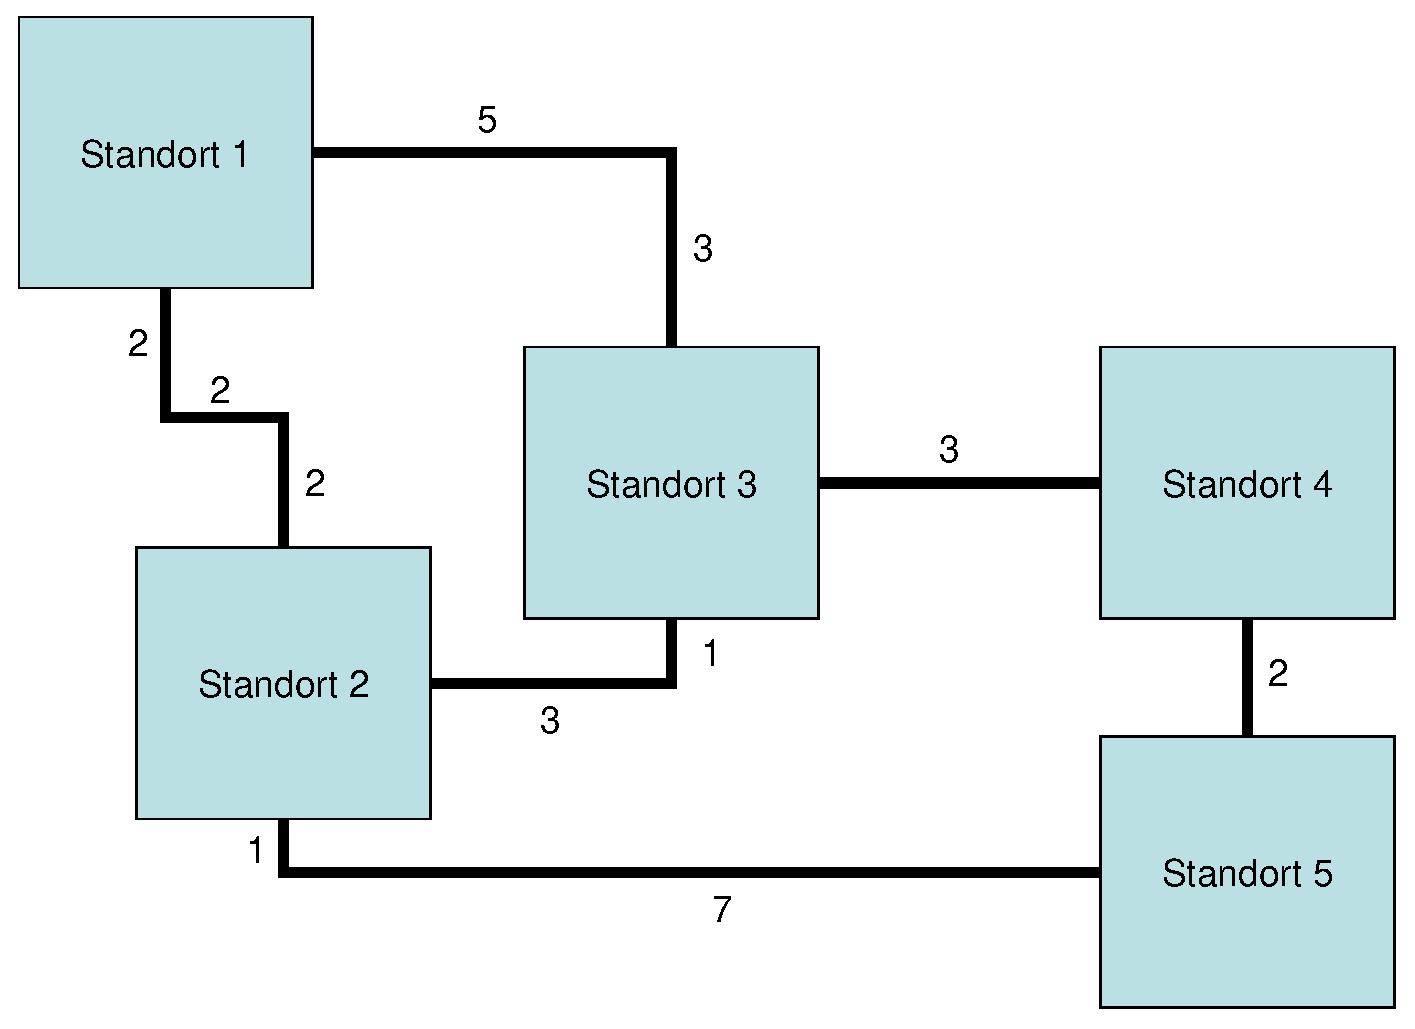
\includegraphics[width=10cm]{images/example_figure}
\caption{An example figure}
\label{fig:example}
\end{center}
\end{figure}

Include only PostScript images (.eps) if you want to create a PostScript document using dvips and only .pdf, .png, .jpeg and .gif images if your goal is a PDF document using pdflatex.
